\chapter{Grundlagen der Computertomographie}\label{grundlagen_bp}

Dieses Kapitel erläutert die für diese Arbeit relevanten theoretischen Grundlagen der Computertomographie. Es werden
zunächst die mathematischen Voraussetzungen gezeigt, darauf aufbauend schließt sich die Beschreibung des \gls{fdk} an.

\section{Mathematische Grundlagen}

In diesem Abschnitt werden die mathematischen Grundlagen der Computertomographie behandelt. Es werden zunächst die
mathematischen Eigenschaften der Vorwärtsprojektion und das sich daraus ergebende Fourier-Schichten-Theorem dargestellt.
Anschließend wird das Prinzip der daraus abgeleiteten gefilterte Rückprojektion erläutert.

\subsection{Projektionen}

Durchquert ein Röntgenstrahl ein festes Objekt, wie beispielsweise biologisches Gewebe oder ein Metall, so wird dieser
Strahl je nach Dichte des Materials entlang seiner Bahn abgeschwächt bzw.\ absorbiert. Mathematisch lässt sich ein
Objekt daher als zwei- oder dreidimensionale Verteilung von linearen Röntgenschwächungskoeffizienten verstehen. Die
Schwächung entlang eines Röntgenstrahls kann als Kurvenintegral dargestellt werden.

Die Grundlage der folgenden Ausführungen ist die Abbildung~\ref{fig:math_proj}. Als Beispiel dienen ein \gls{obj}, hier
durch die Funktion $f(x, y)$ repräsentiert, sowie Kurvenintegrale mit dem Parameterpaar $(\theta, t)$. Die Linie $AB$
lässt sich dann wie folgt darstellen:

\begin{equation*}
    x \cdot \cos \theta + y \cdot \sin \theta  = t_1
\end{equation*}

oder allgemein für beliebige, zu $AB$ parallele, Linien:

\begin{equation}\label{eq:proj_obj}
    x \cdot \cos \theta + y \cdot \sin \theta = t
\end{equation}

\begin{figure}[!htb]
\centering
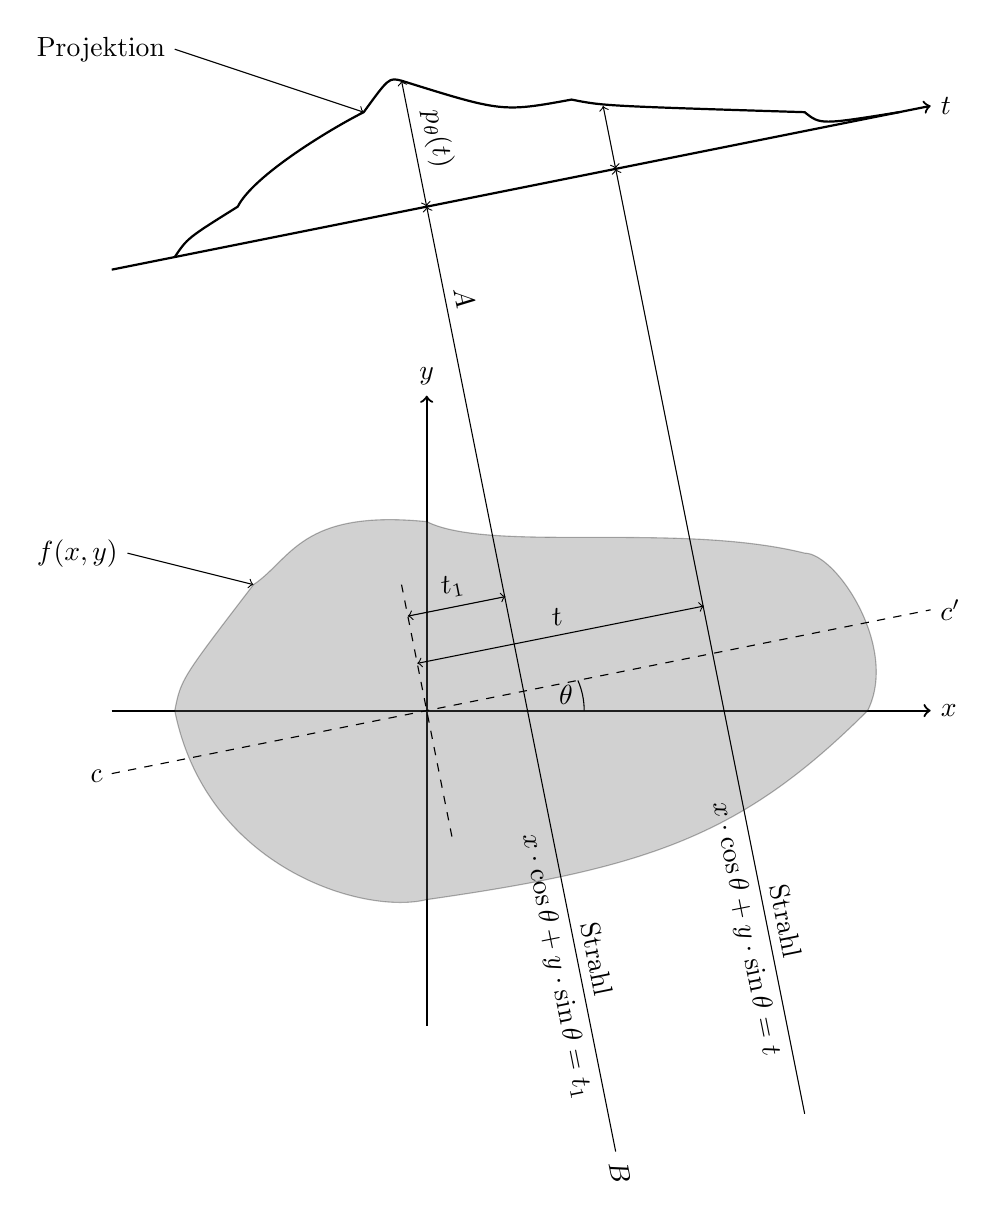
\begin{tikzpicture}[
    scale=0.8,
    axis/.style={thick,->}]
    % Achsen
    \draw[axis] (-5, 0) -- (8, 0) node[right] {$x$};
    \draw[axis] (0, -5) -- (0, 5) node[above] {$y$};
    \draw[axis] (-5, 7) -- (8, 9.6) node[right,sloped] {$t$};

    % Objekt
    \draw[fill=black!60!white,opacity=0.3] (0, -3) .. controls (3.5, -2.5) and (5, -2) .. (7, 0)
                                            .. controls (7.5, 1) and (6.5, 2.5) .. (6, 2.5)
                                            .. controls (4, 3) and (1, 2.5) .. (0,3)
                                            .. controls (-2, 3.2) and (-2.15, 2.4) .. (-2.75, 2)
                                            .. controls (-3.9, 0.5) .. (-4, 0)
                                            .. controls (-3.5, -2.5)  and (-1, -3.25) .. (0, -3);

    % Strahlen
    \draw[->] (3, -7) -- (0, 8) node[pos=0.9,above,sloped] {$A$} node[pos=0.2,above,sloped] {Strahl}
              node[pos=0.2,below,sloped] {$x \cdot \cos \theta + y \cdot \sin \theta = t_1$}
              node[pos=0,right,sloped] {$B$};

    \draw[->] (6, -6.4) -- (3, 8.6) node[pos=0.2,above,sloped] {Strahl}
              node[pos=0.2,below,sloped] {$x \cdot \cos \theta + y \cdot \sin \theta = t$};

    % t
    \draw[<->] (-0.3, 1.5) -- (1.25, 1.81) node[pos=0.5,above,sloped] {$t_1$};
    \draw[<->] (-0.15, 0.75) -- (4.4, 1.66) node[pos=0.5,above,sloped] {$t$};

    % sonstiges
    \draw[dashed] (-5, -1) -- (8, 1.6) node[pos=0,sloped,left] {$c$} node[sloped,right] {$c'$};
    \draw[dashed] (0.4, -2) -- (-0.4, 2);

    % Projektion
    \draw[<->] (0, 8) -- (-0.4, 10) node[pos=0.5, sloped, above] {$p_{\theta}(t)$};
    \draw[<->] (3, 8.6) -- (2.8, 9.6);
    \draw[thick] (-4, 7.2) .. controls (-3.8, 7.5) .. (-3, 8)
                 .. controls (-2.75, 8.5) and (-1.5, 9.25) .. (-1, 9.5)
                 .. controls (-0.6, 10.05) .. (-0.4, 10)
                 .. controls (1.2, 9.5) .. (2.3, 9.7)
                 .. controls (2.8, 9.6) .. (6, 9.5)
                 .. controls (6.25, 9.3) .. (7.5, 9.5);

    % Beschriftungen
    \draw[->] (-4.75, 2.5) -- (-2.75, 2) node[pos=0,left] {$f(x, y)$};
    \draw[->] (-4, 10.5) -- (-1, 9.5) node[pos=0, left] {Projektion};

    % Winkel
    \draw (2.5, 0) arc (0:23.5:12mm) node[pos=0.5,left] {$\theta$};
\end{tikzpicture}
\caption{Zusammenhang zwischen Kurvenintegral und Projektion (Vorlage:~\cite{kak79})}
\label{fig:math_proj}
\end{figure}

Das zu $f(x, y)$ gehörige Kurvenintegral ist $p_{\theta}(t)$:

\begin{equation}\label{eq:proj_int}
    p_{\theta}(t) = \int\limits_{(\theta, t)\text{-Linie}} f(x, y)\ \mathrm{d}s
\end{equation}

Wird die Objektfunktion $f(x, y)$ entlang einer Linie nach Gleichung~\ref{eq:proj_obj} abgetastet, dann lässt sich das
Kurvenintegral wie folgt umschreiben:

\begin{equation}\label{eq:proj_radon}
    p_{\theta}(t) = \int\limits_{-\infty}^{\infty}\int\limits_{-\infty}^{\infty}f(x, y) \cdot \delta(x \cdot
                    \cos \theta + y \cdot \sin \theta - t)\ \mathrm{d} x\ \mathrm{d} y
\end{equation}

Die Funktion $p_{\theta}(t)$ ist die \textit{Radon-Transformation} der Funktion $f(x, y)$ (vgl.~\cite{radon}).

Eine \gls{proj} lässt sich als eine Menge von Radon-Transformationen verstehen. Die (mathematisch) einfachste
\gls{proj} ist eine Sammlung von Parallelstrahlintegralen $p_{\theta}(t)$ unter einem konstanten Winkel $\theta$. Man
bezeichnet eine solche \gls{proj} als \textit{Parallelstrahlprojektion} (siehe Abbildung~\ref{fig:par_proj}). In der
Praxis kann eine Parallelstrahlprojektion durch die Bewegung einer Quelle-Detektor-Anordnung entlang paralleler Linien
auf entgegengesetzten Seiten des \gls{obj}s aufgenommen werden.

Eine zweite Aufnahmemöglichkeit ist der Einsatz einer Quelle auf einer festen Position sowie einer Reihe von Detektoren
entlang einer Linie auf der anderen Seite des \gls{obj}s (siehe Abbildung~\ref{fig:fan_proj}). Solcherart erzeugte
\glspl{proj} nennt man aufgrund der fächerförmigen Strahlen \textit{Fächerstrahlprojektionen}. (vgl.~\cite{kakslan},
S. 49 -- 51)

\begin{figure}
    \centering
    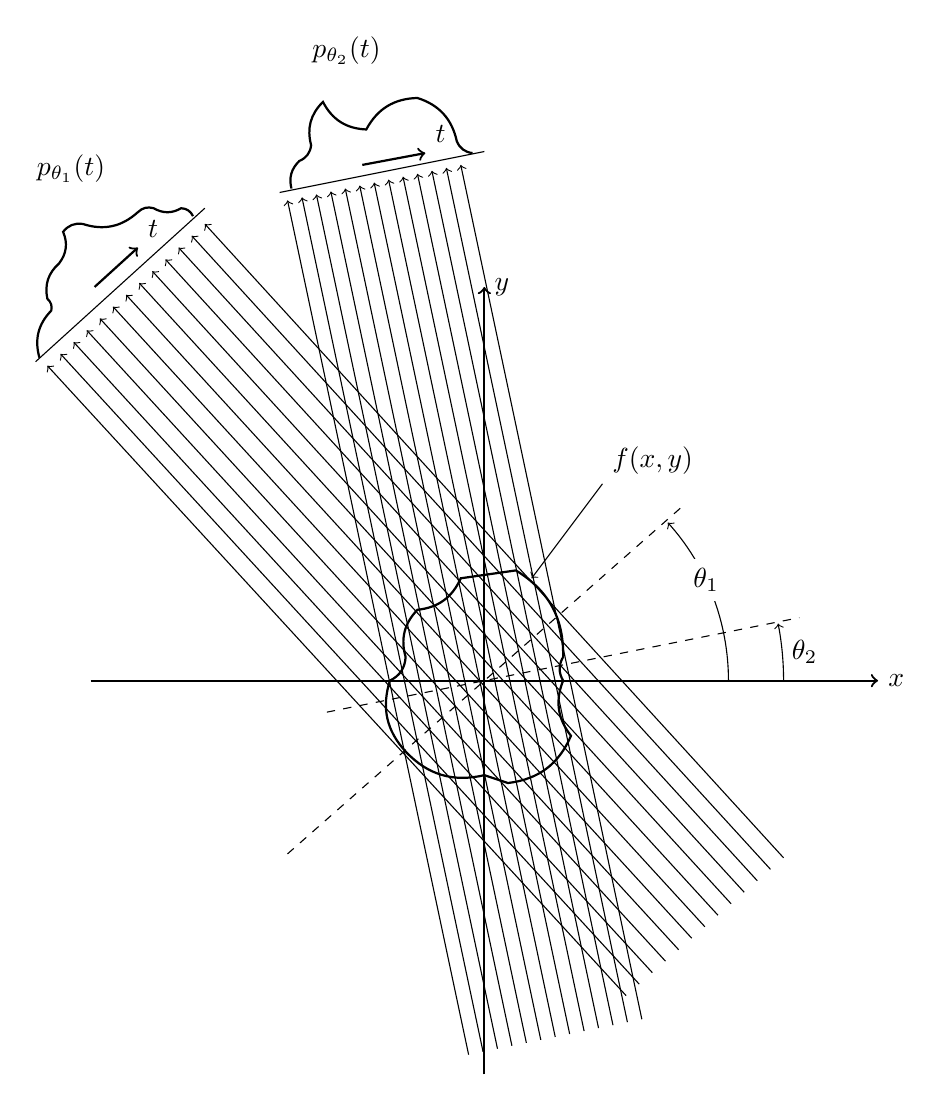
\begin{tikzpicture}[axis/.style={thick,->}]
        \draw[axis] (-5, 0) -- (5, 0) node [right] {$x$};
        \draw[axis] (0, -5) -- (0, 5) node [right] {$y$};

        % Objekt
        \draw[thick] (1, 0) to [bend left] (1, 0.3) to [bend right] (0.4, 1.4) to (-0.3, 1.3)
                     to [bend left] (-0.85, 0.9) to [bend right] (-1, 0.3) to [bend left] (-1.2, 0)
                     to [bend right] (-1, -0.9) to [bend right] (0, -1.2) to (0.3, -1.3) to [bend right] (1.1 ,-0.7)
                     to [bend left] (1, 0);
        \draw[->] (1.5, 2.5) -- (0.6, 1.3) node [pos=0, above right] {$f(x, y)$};

        % Detektorebenen
        \draw[dashed] (-2.5, -2.2) -- (2.5, 2.2);
        \draw[dashed] (-2, -0.4) -- (4, 0.8);

        % Detektor 1
        \draw (-5.7, 4.05) -- (-3.55, 6);
        \draw[axis] (-4.95, 5) -- (-4.4, 5.5) node [sloped, above right] {$t$};
        \draw[thick] (-5.65, 4.1) to [bend left] (-5.5, 4.7) to [bend right] (-5.55, 4.85)
                                  to [bend left] (-5.4, 5.3) to [bend right] (-5.35, 5.7)
                                  to [bend left] (-5.1, 5.8) to [bend right] (-4.4, 5.95)
                                  to [bend left] (-4.2, 6) to [bend right] (-3.85, 6)
                                  to [bend left] (-3.7, 5.9);
        \node at (-5.25, 6.5) {$p_{\theta_1}(t)$};

        % Strahlen zu Detektor 1
        \foreach \w in {0,...,12}
            \draw [->] (1.8 + \w * 0.16666666666667, -4 + \w * 0.14583333333333)
                        -- (-5.55 + \w * 0.16666666666667, 4 + \w * 0.15);

        % Detektor 2
        \draw (-2.6, 6.2) -- (0, 6.72);
        \draw[axis] (-1.55, 6.55) -- (-0.75, 6.7) node [above right] {$t$};
        \draw[thick] (-2.45, 6.25) to [bend left] (-2.35, 6.6) to [bend right] (-2.2, 6.8)
                                   to [bend left] (-2.05, 7.35) to [bend right] (-1.5, 7)
                                   to [bend left] (-0.85, 7.4) to [bend left] (-0.35, 6.85)
                                   to [bend right] (-0.15, 6.7);
        \node at (-1.75, 8) {$p_{\theta_2}(t)$};

        % Strahlen zu Detektor 2
        \foreach \w in {0,...,12}
            \draw [->] (-0.2 + \w * 0.1833333333333, -4.75 + \w * 0.0375)
                        -- (-2.5 + \w * 0.1833333333333, 6.1 + \w * 0.0375);

        % Winkel
        \draw [->] (3.1, 0) arc (0:42:30mm) node [pos=0.6, fill=white] {$\theta_1$};
        \draw [->] (3.8, 0) arc (0:11:38mm) node [pos=0.5, right] {$\theta_2$};
    \end{tikzpicture}
    \caption{Parallelstrahlprojektionen (Vorlage:~\cite{rosenkak}, S. 356)}
    \label{fig:par_proj}
\end{figure}


\begin{figure}
    \centering
    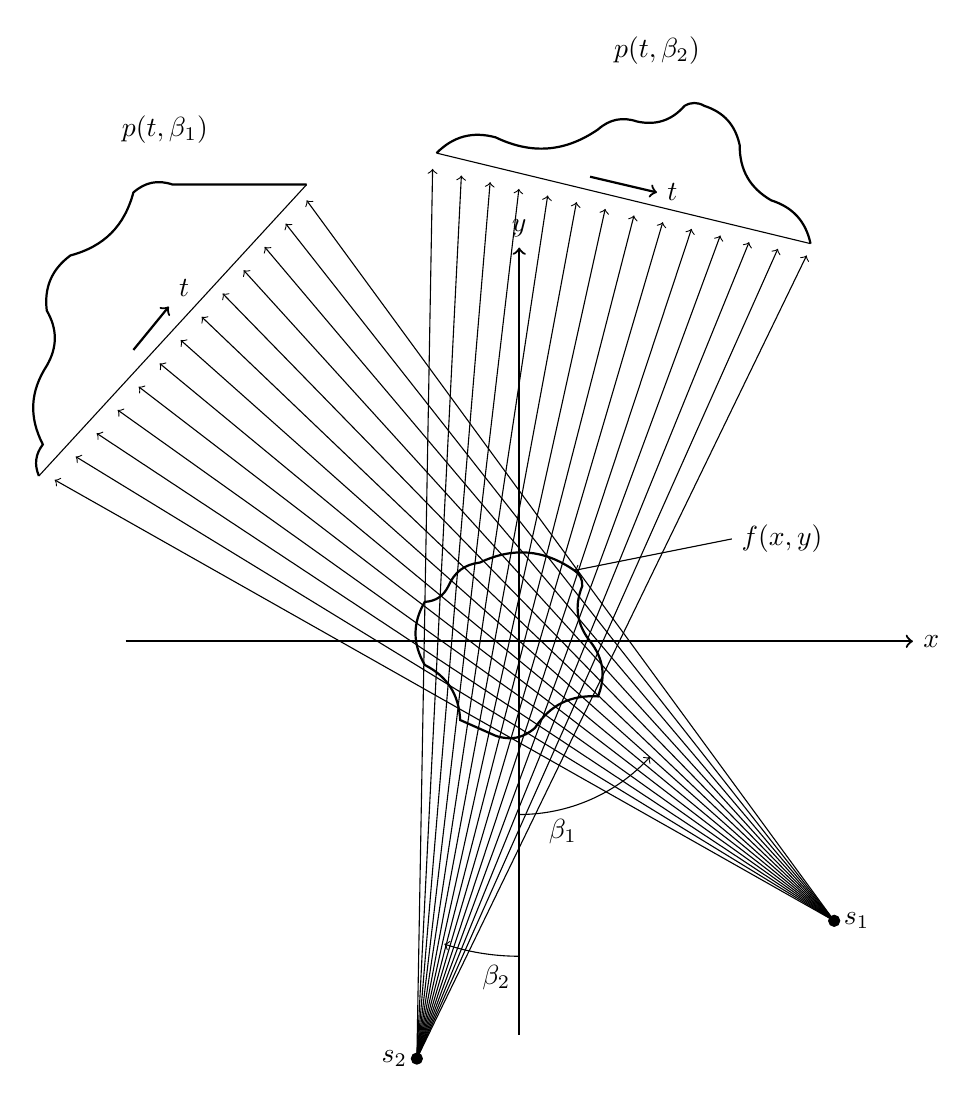
\begin{tikzpicture}[axis/.style={thick,->}]
        \draw[axis] (-5, 0) -- (5, 0) node [right] {$x$};
        \draw[axis] (0, -5) -- (0, 5) node [above] {$y$};

        % Objekt
        \draw[thick] (0.9, 0) to [bend left] (0.8, 0.7) to [bend right] (0.7, 0.9) to [bend right] (-0.5, 1)
                              to [bend right] (-0.9, 0.7) to [bend left] (-1.2, 0.5)
                              to [bend right] (-1.2, -0.3) to [bend left] (-0.75, -1) to (-0.3, -1.2)
                              to [bend right] (0.2, -1.1) to [bend left] (1, -0.7) to [bend right] (0.9, 0.0);
        \draw[->] (2.7, 1.3) -- (0.7, 0.9) node [pos=0, right] {$f(x, y)$};

        % Quellen
        \coordinate (s1) at (4, -3.55);
        \coordinate (s2) at (-1.3, -5.3);
        \draw[fill=black] (s1) circle (2pt) node [right] {$s_1$};
        \draw[fill=black] (s2) circle (2pt) node [left] {$s_2$};

        % Detektor 1
        \draw (-6.1, 2.1) -- (-2.7, 5.8);
        \draw[axis] (-4.9, 3.7) -- (-4.45 , 4.25) node [above right] {$t$};
        \draw[thick] (-6.1, 2.1) to [bend left] (-6.05, 2.5) to [bend left] (-6, 3.5) to [bend right] (-6, 4.2)
                                 to [bend left] (-5.7, 4.9) to [bend right] (-4.9, 5.7) to [bend left] (-4.4, 5.8)
                                 to (-2.7, 5.8);
        \node at (-4.5, 6.5) {$p(t, \beta_1)$};

        % Strahlen zu Detektor 1
        \foreach \w in {0,...,12}
            \draw[->] (s1) -- (-5.9 + \w * 0.266666666666, 2.05 + \w * 0.295833333333333);

        % Detektor 2
        \draw (-1.05, 6.2) -- (3.7, 5.05);
        \draw[axis] (0.9, 5.9) -- (1.75, 5.7) node [right] {$t$};
        \draw[thick] (-1.05, 6.2) to [bend left] (-0.3, 6.4) to [bend right] (1, 6.5) to [bend left] (1.5, 6.6)
                                  to [bend right] (2.1, 6.8) to [bend left] (2.35, 6.8) to [bend left] (2.8, 6.3)
                                  to [bend right] (3.2, 5.6) to [bend left] (3.7, 5.05);
        \node at(1.75, 7.5) {$p(t, \beta_2)$};

        % Strahlen zu Detektor 2
        \foreach \w in {0,...,13}
            \draw[->] (s2) -- (-1.1 + \w * 0.36538415384, 6 - \w * 0.084615384);

        % Winkel
        \draw[->] (0, -2.2) arc (270:317.5:22.5mm) node[pos=0.3,below] {$\beta_1$};
        \draw[->] (0, -4) arc (270:251.5:30mm) node[pos=0.3,below] {$\beta_2$};
    \end{tikzpicture}
    \caption{Fächerstrahlprojektionen (Vorlage:~\cite{rosenkak}, S. 357)}
    \label{fig:fan_proj}
\end{figure}

\subsection{Das Fourier-Scheiben-Theorem}\label{ssec:fourier_scheibe}

Das Fourier-Scheiben-Theorem beschreibt den mathematischen Zusammenhang zwischen der Menge der Projektionen und der
zweidimensionalen Objektfunktion im Ortsraum. Die Fouriertransformation einer Parallelstrahlprojektion eines
\gls{obj}s $f(x, y)$, die unter dem Winkel $\theta$ aufgenommen wurde, entspricht einer Schicht des zweidimensional
fouriertransformierten \gls{obj}s $F(u, v)$.
Mit anderen Worten ergibt die Fouriertransformation einer \gls{proj} $p_{\theta}(t)$ die Werte von $F(u, v$) entlang
einer radialen Linie $BB$ (siehe Abbildung~\ref{fig:fourier_scheibe}). (vgl.~\cite{rosenkak}, S.366)

Dieser Zusammenhang lässt sich auch mathematisch herleiten (siehe Anhang~\ref{app:fourier_scheibe}). Aus ihm folgt, dass
sich die Werte von $F(u, v)$ entlang radialer Linien dadurch bestimmen lassen, dass man die \glspl{proj} des \gls{obj}s
unter mehreren Winkeln $\theta_1$, $\theta_2$, \ldots, $\theta_k$ aufnimmt und diese fouriertransformiert. Für eine
unendliche Anzahl von \glspl{proj} wäre $F(u, v)$ somit in allen Punkten der $uv$-Ebene bestimmt, sodass die
Objektfunktion $f(x, y)$ durch die inverse Fouriertransformation bestimmt werden kann. 
\begin{figure}
    \centering
    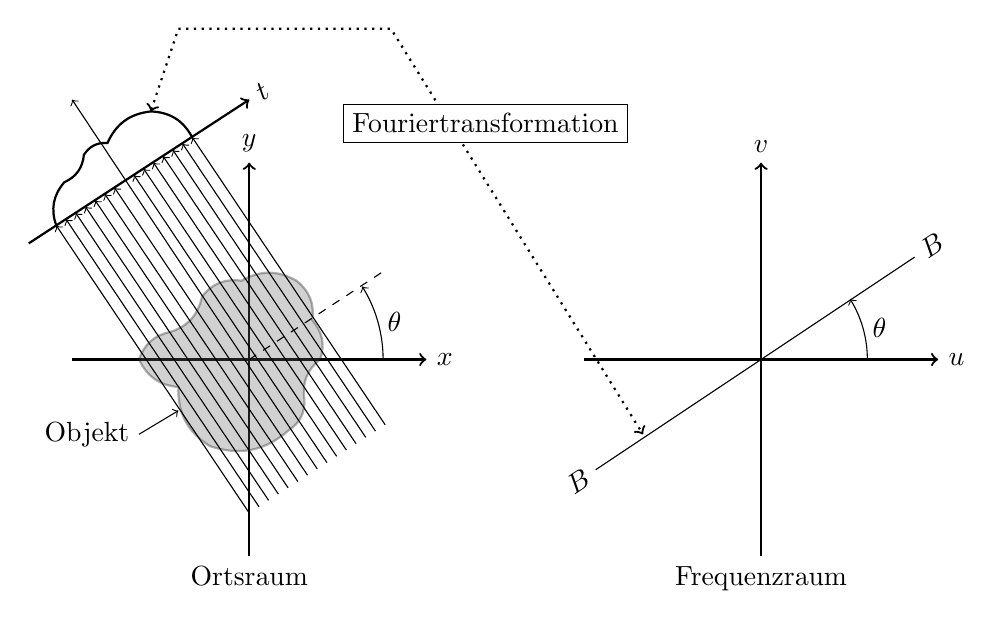
\begin{tikzpicture}[axis/.style={thick,->}]
        % links
        \draw[axis] (-5.5, 0) -- (-1, 0) node [right] {$x$};
        \draw[axis] (-3.25, -2.5) -- (-3.25, 2.5) node[pos=0,below] {Ortsraum} node [above] {$y$};

        % Objekt
        \draw[thick,fill=black!60!white,opacity=0.3] (-2.35, 0) to [bend right] (-2.45, 0.5) to [bend right] (-2.65, 1)
                                                                to [bend right] (-3.35, 1) to [bend right] (-3.85, 0.8)
                                                                to [bend left] (-4.25, 0.35) to [bend right] (-4.65, 0)
                                                                to [bend right] (-4.15 ,-0.35)
                                                                to [bend right] (-3.75, -1.1)
                                                                to [bend right] (-2.75, -0.9)
                                                                to [bend right] (-2.55 ,-0.5)
                                                                to [bend left] (-2.35, 0);
        \draw[->] (-4.65, -0.95) -- (-4.15, -0.65) node[pos=0, left] {Objekt};

        % Detektor
        \draw[axis] (-6.05, 1.475) -- (-3.25, 3.3) node[pos=1,sloped,right] {$t$};
        \draw[thick] (-5.7, 1.7) to [bend left] (-5.6, 2.25) to [bend right] (-5.35, 2.6)
        to [bend left] (-5.05, 2.75) to [bend left] (-4.5, 3.15)
        to [bend left] (-3.9733333333333, 2.82);

        % Pfeile zum Detektor
        \foreach \w in {0,...,6}
            \draw[->] (-3.25 + \w * 0.1233333333333, -1.95 + \w * 0.08)
                      -- (-5.7 + \w * 0.1233333333333, 1.7 + \w * 0.08);
        \draw[->] (-3.25 + 7 * 0.1233333333333, -1.95 + 7 * 0.08) -- (-5.5, 3.3);
        \foreach \w in {8,...,14}
            \draw[->] (-3.25 + \w * 0.1233333333333, -1.95 + \w * 0.08)
                      -- (-5.7 + \w * 0.1233333333333, 1.7 + \w * 0.08);

        % Linie
        \draw[dashed] (-3.25, 0) -- (-1.5, 1.15);

        % Winkel
        \draw[->] (-1.55, 0) arc(0:32:17.5mm) node[pos=0.5,right] {$\theta$};

        % rechts
        \draw[axis] (1, 0) -- (5.5, 0) node [right] {$u$};
        \draw[axis] (3.25, -2.5) -- (3.25, 2.5) node [pos=0,below] {Frequenzraum} node [above] {$v$};

        % Linie
        \draw (1.15, -1.4) -- (5.2, 1.3) node[sloped,pos=0,left] {$B$} node[sloped,pos=1,right] {$B$};

        % Winkel
        \draw[->] (4.6, 0) arc (0:32:14.5mm) node[pos=0.5,right] {$\theta$};

        % Verbindung
        \draw[<->,dotted,thick] (-4.5, 3.15) -- (-4.15, 4.2) -- (-1.45, 4.2) -- (1.75, -0.95);
        \node[draw,fill=white] at (-0.25, 3) {Fouriertransformation};
    \end{tikzpicture}
    \caption{Das Fourier-Scheiben-Theorem (Vorlage:~\cite{kakslan}, S. 57)}
    \label{fig:fourier_scheibe}
\end{figure}

\begin{figure}
    \centering
    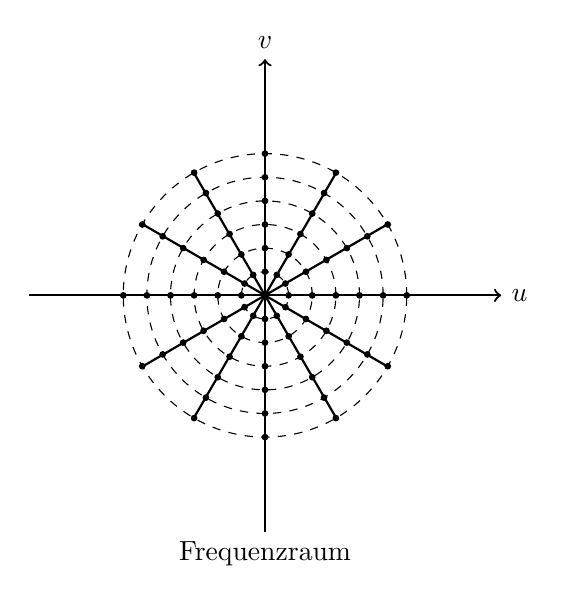
\begin{tikzpicture}[axis/.style={thick,->}]
        \draw[axis] (-3, 0) -- (3, 0) node [right] {$u$};
        \draw[axis] (0, -3) -- (0, 3) node[pos=0,below] {Frequenzraum} node [above] {$v$};

        % Kreise
        \draw[dashed] (0, 0) circle (3mm);
        \draw[dashed] (0, 0) circle (6mm);
        \draw[dashed] (0, 0) circle (9mm);
        \draw[dashed] (0, 0) circle (12mm);
        \draw[dashed] (0, 0) circle (15mm);
        \draw[dashed] (0, 0) circle (18mm);

        % Linien
        \draw[thick] (-1.55, -0.9) -- (1.55, 0.9);
        \draw[thick] (-0.9, -1.55) -- (0.9, 1.55);
        \draw[thick] (0.9, -1.55) -- (-0.9, 1.55);
        \draw[thick] (1.55, -0.9) -- (-1.55, 0.9);

        % Punkte
        \foreach \w in {0,...,6}
            \draw[fill=black] (0, 0 + \w * 0.3) circle (1pt);
        \foreach \w in {0,...,6}
            \draw[fill=black] (0, 0 - \w * 0.3) circle (1pt);

        \foreach \w in {0,...,6}
            \draw[fill=black] (0 + \w * 0.3, 0) circle (1pt);
        \foreach \w in {0,...,6}
            \draw[fill=black] (0 - \w * 0.3, 0) circle (1pt);

        \foreach \w in {0,...,6}
            \draw[fill=black] (30:\w * 3mm) circle (1pt);
        \foreach \w in {0,...,6}
            \draw[fill=black] (60:\w * 3mm) circle (1pt);
        \foreach \w in {0,...,6}
            \draw[fill=black] (120:\w * 3mm) circle (1pt);
        \foreach \w in {0,...,6}
            \draw[fill=black] (150:\w * 3mm) circle (1pt);
        \foreach \w in {0,...,6}
            \draw[fill=black] (210:\w * 3mm) circle (1pt);
        \foreach \w in {0,...,6}
            \draw[fill=black] (240:\w * 3mm) circle (1pt);
        \foreach \w in {0,...,6}
            \draw[fill=black] (300:\w * 3mm) circle (1pt);
        \foreach \w in {0,...,6}
            \draw[fill=black] (330:\w * 3mm) circle (1pt);
    \end{tikzpicture}
    \caption{Radiale Linien, entstanden durch fouriertransformierte Projektionen (Vorlage:~\cite{kakslan}, S. 59)}
    \label{fig:fourier_scheibe_endlich}
\end{figure}

\subsection{Die gefilterte Rückprojektion}\label{ssec:filter_bp}

Durch das Fourier-Scheiben-Theorem lassen sich ein \gls{fourobj} und eine \gls{fourproj} entlang einer radialen Linie in
einen Zusammenhang stellen. Daraus folgt, dass man mit genügend vielen fouriertransformierten \glspl{proj}, die unter
unterschiedlichen Winkeln aufgenommen wurden, das zweidimensional fouriertransformierte \gls{obj} und damit (durch die
inverse Fouriertransformation) das \gls{obj} selbst rekonstruieren kann. Dieses einfache Modell der Tomographie lässt
sich jedoch nur mit viel Aufwand in dieser Form implementieren. (vgl.~\cite{kakslan}, S. 60)

Ein bekannter Ansatz, der weniger Aufwand erfordert, ist die gefilterte Rückprojektion, die sich aus dem
Fourier-Scheiben-Theorem herleiten lässt. Dazu werde die inverse Fouriertransformation in einem polaren
Koordinatensystem durchgeführt und die Grenzen der zugehörigen Integrale entsprechend angepasst (zur mathematischen
Herleitung siehe~\cite{kakslan}, S. 63 -- 68). Es ist dieser Schritt, der eine effiziente Implementierung der
Rekonstruktion für Computer ermöglicht; Kak und Slaney stellen fest: {\glqq}The derivation of this algorithm is perhaps
one of the most illustrative examples of how we can obtain a radically different computer implementation by simply
rewriting the fundamental expressions for the underlying theory{\grqq} (siehe~\cite{kakslan}, S. 60).

Die Grundlage der gefilterten Rückprojektion ist der Umstand, dass jede \gls{proj} eine nahezu unabhängige Aufnahme des
\gls{obj}s darstellt. Die einzige Gemeinsamkeit der unter verschiedenen Winkeln aufgenommenen \glspl{proj} ist die
Gleichheit im Punkt $F(0, 0)$. Transformiert man eine einzelne \gls{proj} und nimmt an, dass es keine anderen
\glspl{proj} gibt, so lässt sich durch die zweidimensionale inverse Fouriertransformation ein (verzerrtes) \gls{obj}
rekonstruieren. Es kann gezeigt werden (vgl.~\cite{kakslan}, S. 61), dass eine solche Rekonstruktion äquivalent der mit
einem einfachen Filter multiplizierten Fouriertransformierten der originalen Objektfunktion ist. Durch das Aufsummieren
mehrerer transformierter \glspl{proj} ergibt sich schließlich das rekonstruierte \gls{obj}. Da die Fouriertransformation
eine lineare Operation ist, lässt sich dieses Aufsummieren der \glspl{proj} auch im Ortsraum durchführen. In diesem Fall
spricht man von der Rückprojektion. (vgl.~\cite{kakslan}, S. 61)

Die Filterung lässt sich als Wichtung der \glspl{proj} im Frequenzraum betrachten. Wie bereits in
Abschnitt~\ref{ssec:fourier_scheibe} erwähnt, nimmt die Dichte der (in endlicher Zahl vorliegenden) bekannten
Punkte im Frequenzraum mit steigender Distanz zum Ursprung ab. Durch die stärkere Wichtung der höheren Frequenzen der
\glspl{proj} lassen sich die fehlenden Punkte approximieren, durch eine möglichst hohe Projektionszahl lässt sich die
durch die fehlenden Informationen hervorgerufene Abweichung weiter verringern. (vgl.~\cite{kakslan}, S. 61)

Die gewichteten \glspl{proj} lassen sich (im Anschluss an die inverse Fouriertransformation) aufsummieren, um das
\gls{obj} zu rekonstruieren. Zusammengefasst ergibt sich für die gefilterte Rückprojektion der folgende Algorithmus:

Für alle Winkel $\theta$:
\begin{enumerate}
    \item \gls{proj} $p_{\theta}(t)$ aufnehmen
    \item $p_{\theta}(t)$ zu $P_{\theta}(w)$ fouriertransformieren
    \item $P_{\theta}(w)$ filtern
    \item $P_{\theta}(w)$ invers fouriertransformieren und zurückprojizieren (Addition zum bisherigen Ergebnis)
\end{enumerate}

Dieser Algorithmus bietet den Vorteil, dass direkt nach dem Aufnehmen der ersten \gls{proj} begonnen werden kann.
Daneben ist es einfacher, im Ortsraum zu interpolieren, als wenn man dies im Frequenzraum täte, da im Ortsraum eine
lineare Interpolation häufig genügt. (vgl.~\cite{kakslan}, S. 62)

\section{Der Feldkamp-Davis-Kress-Algorithmus}\label{sec:fdk}

Der 1984 entwickelte \gls{fdk}~\cite{fdk} ist eine spezielle Ausprägung der gefilterten Rückprojektion für die
Computertomographie mit Kegelstrahlen. In diesem Abschnitt wird zunächst die zugrundeliegende Mathematik näher
erläutert, bevor die einzelnen Schritte des \gls{fdk} detaillierter betrachtet werden.

\subsection{Grundlagen}\label{ssec:fdk_math}

Die Idee des \gls{fdk} ist die Erweiterung der in Abschnitt~\ref{ssec:filter_bp} vorgestellten gefilterten
Rückprojektion auf die dritte Dimension. Ausgangspunkt ist eine Fächerstrahlprojektion (siehe
Abbildung~\ref{fig:fan_proj}), die jetzt im dreidimensionalen Raum betrachtet wird, wie in
Abbildung~\ref{fig:fdk_schema} dargestellt. Ausgehend von der Schnittgeraden der mittleren Ebene ($z = 0$) mit der
Detektorebene, also der Projektion, lassen sich die in der mittleren Ebene liegenden Punkte rekonstruieren. Verschiebt
man nun die Schnittgerade (den Fächer) bei gleichbleibender Quellposition derart, dass sie parallel zur Schnittgeraden
der mittleren Ebene mit dem Detektor bleibt (konstantes $z$, $z \neq 0$), so befinden sich die so erfassten Punkte
ebenfalls innerhalb einer Ebene. Diese neue Ebene lässt sich ebenfalls als eine mittlere Ebene betrachten, die
allerdings im Vergleich zur {\glqq}ursprünglichen{\grqq} mittleren Ebene gekippt ist.

Um die Rückprojektion einer Fächerstrahlprojektion auf die gekippte Ebene anwenden zu können, müssen die durch die
Verschiebung entstandenen Veränderungen berücksichtigt werden. Zum Aufnahmewinkel der Projektion kommt nun noch der
Winkel zwischen der gekippten Ebene und der mittleren Ebene hinzu, außerdem hat sich für den gekippten Strahl die
Distanz zwischen der Quelle und dem Detektor vergrößert. Rechnet man diese Faktoren mit ein, so lässt sich die
Rückprojektion von Fächerstrahlprojektionen auch im dreidimensionalen Raum durchführen (zur mathematischen Herleitung
siehe~\cite{fdk}, S. 614 -- 615). Aufgrund der Kegelform der von der Quelle ausgehenden Strahlen bezeichnet man sie auch
als \textit{Kegelstrahlen} (englisch \textit{cone-beam}; vgl.\ den Titel der Arbeit von Feldkamp, Davis und Kress,
\textit{Practical cone-beam algorithm}).

Es ist zu beachten, dass die Kegelstrahltomographie, sofern sie nur auf einer Kreisbahn um das Objekt herum erfolgt,
mathematisch unterbestimmt ist. Infolgedessen bietet der von diesem Fall ausgehende \gls{fdk} keine exakte, sondern
nur eine näherungsweise Lösung: {\glqq}No rigorous proof exists [\ldots], since the result is approximate{\grqq}
(siehe~\cite{fdk}, S. 614).

\begin{figure}
    \centering
    \begin{tikzpicture}
        % Detektor
        \draw (3, 4, -4) -- (9, 4, 4) -- (9, -4, 4) -- (3, -4, -4) -- (3, 4, -4);

        % Rotationsachse unten
        \draw (0, -3, 0) -- (0, 0, 0);

        % mittlere Ebene
        \draw[fill=white] (-6, 0, -4) -- (0, 0, 4) -- (9, 0, 4) -- (3, 0, -4) -- (-6, 0, -4);

        % mittlere Achse
        \draw (-3, 0, 0) -- (6, 0, 0);
        \draw[fill=black] (-3, 0, 0) circle (1pt) node [below left] {$(-d_{src}, 0, 0)$};
        \draw[fill=black] (6, 0, 0) circle (1pt) node [above right] {$(d_{det}, 0, 0)$};
        
        % Volumen oben
        \draw[fill=white] (0, 1, -1) -- (-1, 1, -1) -- (0, 1, 1) -- (1, 1, 1) -- (0, 1, -1);
        \draw[fill=white] (0, 0, 1) -- (0, 1, 1) -- (1, 1, 1) -- (1, 0, 1);
        \draw[fill=white] (-1, 0, -1) -- (-1, 1, -1) -- (0, 1, 1) -- (0, 0, 1);

        % Volumen unten
        \draw[dashed] (0, 0, 1) -- (0, -1, 1) -- (1, -1, 1) -- (1, 0, 1);
        \draw[dashed] (-1, -1, -1) -- (-1, 0, -1);
        \draw[dashed] (-1, -1, -1) -- (0, -1, 1);
        \draw[dashed] (0, -1, -1) -- (1, -1, 1);

        % weitere Punkte
        \draw[fill=black] (0, 0, 0) circle (1pt);
        \draw[fill=black] (4, 1, -4) circle (1pt);
        \draw[fill=black] (-0.5, 5/14, -10/7) circle (1pt);

        % Quelle - Detektorpunkt
        \draw (-3, 0, 0) -- (4, 1, -4);

        % Beschriftungen
        \draw[->] (0, 0, 6) -- (0, 0, 3) node [pos=0, below left] {mittlere Ebene};
        \draw[->] (0, 3, -3) -- (4, 2, -4) node [pos=0, left] {Detektorebene};
        \draw[->] (2.5, -1, 0) -- (0, 0, 0) node [pos=0, right] {$(0, 0, 0)$};
        \draw[->] (2.5, 0.5, 0) -- (-0.5, 5/14, -10/7) node[pos=0, right] {$(x, y, z)$};

        % fehlende Linien
        \draw[dashed] (3, 0, -4) -- (3, -4, -4); % Detektor
        \draw[dashed] (0, -2, 0) -- (0, 0, 0); % Rotationsachse unten
        \draw[dashed] (0, 0, 0) -- (0, 1, 0); % Rotationsachse oben 1
        \draw (0, 1, 0) -- (0, 3, 0); % Rotationsachse oben 2
        \draw[dashed] (-1, 0, 0) -- (1, 0, 0); % mittlere Achse

    \end{tikzpicture}
    \caption{Schematische Darstellung eines 3D-Tomographiesystems (Vorlage:~\cite{fdk})}
    \label{fig:fdk_schema}
\end{figure}

\subsection{Geometrie}\label{ssec:fdk_geometrie}

Basierend auf den oben genannten Faktoren lässt sich ein dreidimensionales Tomographiesystem wie in
Abbildung~\ref{fig:fdk_geometrie} darstellen. Der Ausgangspunkt der Strahlung ist eine Quelle $S$, die das Objekt $f$
unter einem Drehwinkel $\theta$ mit einem Kegelstrahl durchleuchtet und auf einem Detektor mit $N_h \cdot N_v$
\gls{pixel}n abbildet. Dabei ist \glssymbol{dsrc} der Abstand zwischen der Quelle und dem Rotationsmittelpunkt, also
dem Zentrum des durchleuchteten Volumens, während \glssymbol{ddet} den Abstand zwischen dem Rotationsmittelpunkt und dem
Detektor darstellt. \glssymbol{dh} und \glssymbol{dv} geben den physischen horizontalen bzw.\ vertikalen Abstand zweier
benachbarter Detektorpixelzentren an, die Breite und Höhe des Detektors lassen sich daher mit $N_h \cdot d_h$ und
$N_v \cdot d_v$ bestimmen.

\begin{figure}[!htb]
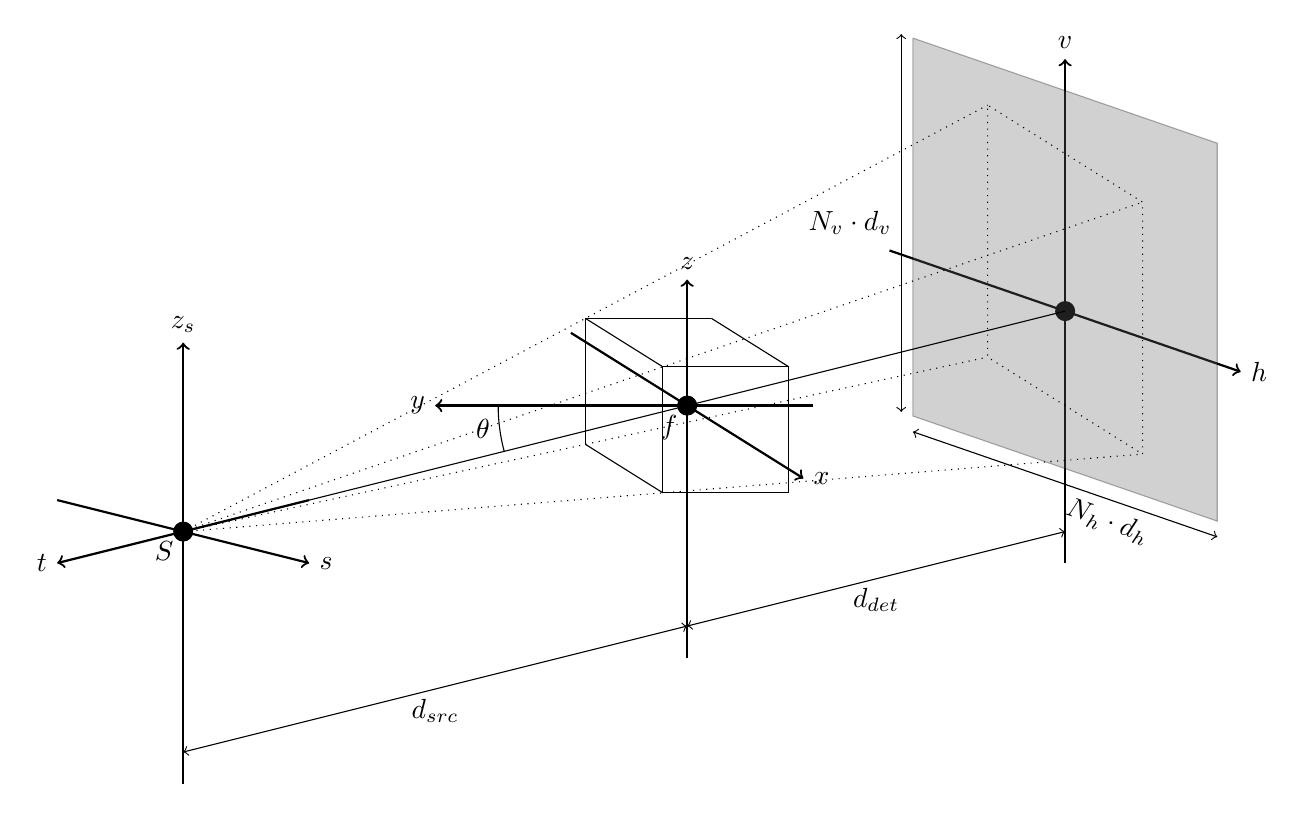
\begin{tikzpicture}[
        scale=0.8,
        axis/.style={thick,->}
    ]
    % Quelle
    \coordinate (1) at (0, 0, 0);
    \filldraw[fill=black,draw=black] (1) circle (0.15cm) node[below left] {$S$};
    \draw[axis] (-2, 0.5, 0) -- (2, -0.5, 0) node[right] {$s$};
    \draw[axis] (2, 0.5, 0) -- (-2, -0.5, 0) node[left] {$t$};
    \draw[axis] (0, -4, 0) -- (0, 3, 0) node[above] {$z_s$};

    % Volumen
    \coordinate (2) at (8, 2, 0);
    \filldraw[fill=black,draw=black] (2) circle (0.15cm) node[below left] {$f$};
    \draw[axis] (5, 2, -3) -- (11, 2, 3) node[right] {$x$};
    \draw[axis] (10, 2, 0) -- (4, 2, 0) node[left] {$y$};
    \draw[axis] (8, -2, 0) -- (8, 4, 0) node[above] {$z$};

    \draw (8, 1, 1) -- (10, 1, 1);
    \draw (8, 1, 1) -- (8, 3, 1);
    \draw (8, 1, 1) -- (6, 1, -1);

    \draw (8, 3, 1) -- (10, 3, 1);
    \draw (8, 3, 1) -- (6, 3, -1);

    \draw (10, 1, 1) -- (10, 3, 1);

    \draw (6, 1, -1) -- (6, 3, -1);

    \draw (6, 3, -1) -- (8, 3, -1);

    \draw (10, 3, 1) -- (8, 3, -1);


    % Detektor
    \coordinate(3) at (14, 3.5, 0);
    \filldraw[fill=black,draw=black] (3) circle (0.15cm);
    \draw[axis] (10.25, 3.5, -2.5) -- (17.75, 3.5, 2.5) node[right] {$h$};
    \draw[axis] (14, -0.5, 0) -- (14, 7.5, 0) node[above] {$v$};
    \draw[fill=black!60!white,opacity=0.3] (10.75, 7, -2.16666) -- (17.25, 7, 2.16666) -- (17.25, 1, 2.16666)
                                           -- (10.75, 1, -2.16666) -- (10.75, 7, -2.16666);
    \draw[<->] (10.5, 1, -2.33333) -- (10.5, 7, -2.33333) node[pos=0.5, left] {$N_v \cdot d_v$};
    \draw[<->] (10.75, 0.75, -2.16666) -- (17.25, 0.75, 2.16666) node[pos=0.5,sloped,below right] {$N_h \cdot d_h$};

    % Abstände
    \draw (1) -- (3);
    \draw[<->] (0, -3.5, 0) -- (8, -1.5, 0) node[pos=0.5,below] {$d_{src}$};
    \draw[<->] (8, -1.5, 0) -- (14, 0, 0) node[pos=0.5,below] {$d_{det}$};

    % Kegelstrahlen
    \draw[dotted] (1) -- (16, 2, 2);
    \draw[dotted] (1) -- (16, 6, 2);
    \draw[dotted] (1) -- (12, 2, -2);
    \draw[dotted] (1) -- (12, 6, -2);

    % Kegelstrahlenabbild
    \draw[dotted] (16, 2, 2) -- (16, 6, 2) -- (12, 6, -2) -- (12, 2, -2) -- (16, 2, 2);

    % Winkel
    \draw (5, 2, 0) arc (180:195:2.8cm) node[pos=0.5, left] {$\theta$};
\end{tikzpicture}
\caption{Geometrie der gefilterten Rückprojektion}
\label{fig:fdk_geometrie}
\end{figure}

\subsection{Wichtung}\label{ssec:fdk_wichtung}

Aufgrund der Kegelform der Strahlung hat jeder Strahl, der das Volumen durchleuchtet, beim Auftreffen auf den Detektor
einen im Vergleich zu den restlichen Strahlen unterschiedlich langen Weg zurückgelegt. Um die durch die
Streckenunterschiede bedingten Absorptionsveränderungen auszugleichen, ist es erforderlich, jeden Punkt der Projektion
(\gls{pixel}) zu wichten.
Dafür wird jedes \gls{pixel} mit den Koordinaten $(j, i)$ mit dem Wichtungsfaktor $w_{ij}$ multipliziert, der auf den
Abständen $d_{src}$ und $d_{det}$ sowie den vertikalen und horizontalen Distanzen des individuellen \gls{pixel}s vom
Ursprung des Detektorkoordinatensystems basiert:

\begin{equation}\label{eq:wichtung}
    w_{ij} = \frac{d_{det} - d_{src}}{\sqrt{(d_{det} - d_{src})^2 + h_j^2 + v_i^2}}
\end{equation}

\subsection{Filterung}\label{ssec:fdk_filter}

Aufgrund der in Abschnitt~\ref{ssec:filter_bp} genannten Gründe müssen die gewichteten Projektionen vor der Rückprojektion
gefiltert werden. Da es sich bei der Kegelstrahltomographie im Wesentlichen um eine erweiterte Fächerstrahltomographie
handelt, genügt es, die Projektionen zeilenweise zu filtern, wie man es bei einem {\glqq}Stapel{\grqq} von
Fächerstrahlprojektionen tun würde. Zu diesem Zweck müssen die Projektionen und der zum Einsatz kommende Filter
fouriertransformiert werden. Da dieses Verfahren nur mit einer Menge von Elementen funktioniert, die einer Zweierpotenz
entspricht, müssen die Projektionszeilen- und die Filtergröße auf die nächste Zweierpotenz erweitert werden. Dazu wird,
ausgehend von der Länge einer Projektionszeile $N_h$, die Filterlänge $N_{hFFT}$ berechnet:

\begin{equation}
    N_{hFFT} = 2 \cdot 2^{\left\lceil \log_{2} N_h \right\rceil}
\end{equation}

Mit der so bestimmten Filterlänge lässt sich ein einfacher Rampenfilter $r$ erzeugen:

\begin{equation}\label{eq:filter_gen}
    \begin{aligned}
        r(j) \text{ mit } j &\in \left[-\frac{N_{hFFT} - 2}{2}, \frac{N_{hFFT}}{2}\right]\\
        r(j) &=
            \begin{cases}
                \frac{1}{8} \cdot \frac{1}{d_h^2} & \quad \text{wenn } j = 0\\
                0 & \quad \text{wenn } j \text{ gerade}\\
                -\frac{1}{2j^2\pi^2d_h^2} & \quad \text{wenn } j \text{ ungerade}\\
            \end{cases}
    \end{aligned}
\end{equation}

Nun wird die zu filternde Zeile so lange mit $0$ aufgefüllt, bis die erweiterte Zeile $N_{hFFT}$ \gls{pixel} umfasst:

\begin{equation}
    \begin{aligned}
        p_0 &: \text{ mit Nullen aufgefüllte Projektionszeile}\\
        p_0(0 \dots N_{h - 1}) &= p(0 \dots N_{h - 1})\\
        p_0(N_{h} \dots N_{hFFT}) &= 0
    \end{aligned}
\end{equation}

Im Anschluss werden sowohl der Filter $r$ als auch die erweiterte Projektionszeile $p_0$ in den Frequenzraum
transformiert und dort miteinander multipliziert:

\begin{equation}
    \begin{aligned}
        R &= \text{FFT}(r)\\
        P &= \text{FFT}(p_0)\\
        P_F &= P \cdot R \quad \text{sowohl für den realen als auch den imaginären Teil}
    \end{aligned}
\end{equation}

Die gefilterte Projektionszeile $P_F$ wird dann mit der inversen schnellen Fouriertransformation (IFFT) in den Ortsraum
zurücktransformiert und von den {\glqq}aufgefüllten{\grqq} Elementen bereinigt:

\begin{equation}
    \begin{aligned}
        p_F &= \text{IFFT}(P_F)\\
        \text{gefilterte Projektionszeile} &: p_F(0 \dots N_{h - 1})
    \end{aligned}
\end{equation}

\subsection{Rückprojektion}\label{sssec:backprojection}

Die gefilterten Projektionen können nun für die Rückprojektion verwendet werden. Dazu werden für jede vorhandene
Projektion $p_F$, die unter dem Drehwinkel $\theta$ aufgenommen wurde, die folgenden Schritte ausgeführt:

\begin{itemize}
    \item berechne für jede \gls{voxel}koordinate $(x, y, z)$ deren Position im rotierten Koordinatensystem
          $(s, t, z)$:
        \begin{equation}
            \begin{aligned}
                s &= x \cos \theta + y \sin \theta\\
                t &= -x \sin \theta + y \cos \theta\\
                z &= z
            \end{aligned}
        \end{equation}

    \item projiziere die rotierte \gls{voxel}koordinate $(s, t, z)$ auf den Detektor:
        \begin{equation}
            \begin{aligned}
                h &= t \cdot \frac{d_{det} - d_{src}}{s - d_{src}}\\
                v &= z \cdot \frac{d_{det} - d_{src}}{s - d_{src}}
            \end{aligned}
        \end{equation}

    \item interpoliere das Detektorsignal bei $(h, v)$:
        \begin{equation}
            \begin{aligned}
                det = p_F(h, v)
            \end{aligned}
        \end{equation}

    \item führe die Rückprojektion für jedes \gls{voxel} $vol_{xyz}$ aus:
        \begin{equation}
            \begin{aligned}
                vol_{xyz} &= vol_{xyz} + 0{,}5 \cdot det \cdot u^2\\
                \text{mit } u &= \frac{d_{src}}{s - d_{src}}
            \end{aligned}
        \end{equation}
\end{itemize}
